\documentclass{ximera}

\newcommand{\RR}{\mathbb R}
\renewcommand{\d}{\,d}
\newcommand{\dd}[2][]{\frac{d #1}{d #2}}
\renewcommand{\l}{\ell}
\newcommand{\ddx}{\frac{d}{dx}}
\newcommand{\dfn}{\textbf}
\newcommand{\eval}[1]{\bigg[ #1 \bigg]}


\author{Jason Miller}
\license{Creative Commons 3.0 By-bC}


\outcome{}

\begin{document}
\begin{exercise}


Consider the polar curve $r=3\sin(2\theta)$. The graph is show below. 




\begin{image}  
  \begin{tikzpicture}  
    \begin{axis}[  
        xmin=-2.5,  
        xmax=2.5,  
        ymin=-2.5,  
        ymax=2.5,  
        axis lines=center,  
        xlabel=$x$,  
        ylabel=$y$,  
        every axis y label/.style={at=(current axis.above origin),anchor=south},  
        every axis x label/.style={at=(current axis.right of origin),anchor=west},  
      ]  
      \addplot [data cs=polar, very thick, mark=none,fill=fill1,domain=0:90,samples=360,smooth] (x, {3*sin(2*x)}) \closedcycle;
      \addplot[data cs=polar,blue,domain=0:360,samples=360,smooth, thick] (x,{3*sin(2*x)});
      
            \end{axis}  
  \end{tikzpicture}  
\end{image} 

We want to determine the area of the shaded region $S$.

The area of the region $S$ is 

\[
\int_{\answer{0 }}^{\answer{ \frac{\pi}{2} }}  \answer{ \frac{1}{2}(3 \sin(2\theta))^2   } \d \theta=\answer{ \frac{9\pi}{8}}
\]


The entire area enclosed by the curve (all four petals) is $\answer{ 4 \frac{9\pi}{8}}$. 


\begin{hint}

Consider a general polar curve $r=f(\theta)$ as below. 


\begin{image}
  \begin{tikzpicture}
\begin{axis}[
axis y line=middle,axis x line=middle,name=myplot,%
			%x=.37\marginparwidth,
			%y=.37\marginparwidth,
			%xtick={-1,1},
			%minor x tick num=1,% 
%			extra x ticks={.33},
%			extra x tick labels={$1/3$},
			%ytick={-1,1},
			%minor y tick num=1,%extra y ticks={-5,-3,...,7},%
			ymin=-.1,ymax=1.1,%
			xmin=-.1,xmax=1.1%
]

\addplot [fill1,fill=fill1,area style, smooth,domain=18:72,samples=30] ({cos(x)*(1+.05*cos(9*x))},{sin(x)*(1+.05*cos(9*x))}) -- (axis cs:0,0) -- cycle;

\addplot [penColor,thick, smooth,domain=0:90,samples=30] ({cos(x)*(1+.05*cos(9*x))},{sin(x)*(1+.05*cos(9*x))});



\draw [thick,penColor,] (axis cs:0,0) -- (axis cs: 0.905831, 0.294322) node [pos=.7,below,rotate=18,black] { $\theta=\alpha$};

\draw [thick,penColor,] (axis cs:0,0) -- (axis cs:0.313792, 0.965751) node [pos=.7,above,rotate=72,black] { $\theta=\beta$};


\draw (axis cs:.8,.85) node { $f(\theta)$};


\end{axis}

\node [right] at (myplot.right of origin) { $0$};
\node [above] at (myplot.above origin) { $\pi/2$};
\end{tikzpicture}
\end{image}


Recall that the area enclosed by a polar curve $r=f(\theta)$ from $\theta=\alpha$ to $\theta=\beta$ is given 

\[
\int_{\alpha}^{\beta} \frac{1}{2} f(\theta)^2 \d \theta
\]


In our case $f(\theta)=3\sin(2\theta)$. So we only need to identify the initial angle $\alpha$ and the final angle $\beta$ that bounds our region $S$. 

In order to determine these angles we need to think about how the curve is traced out as $\theta$ varies. 

Let's graph $r=3\sin(2\theta)$ on $r$ and $\theta$ axes. 

\begin{image}  
  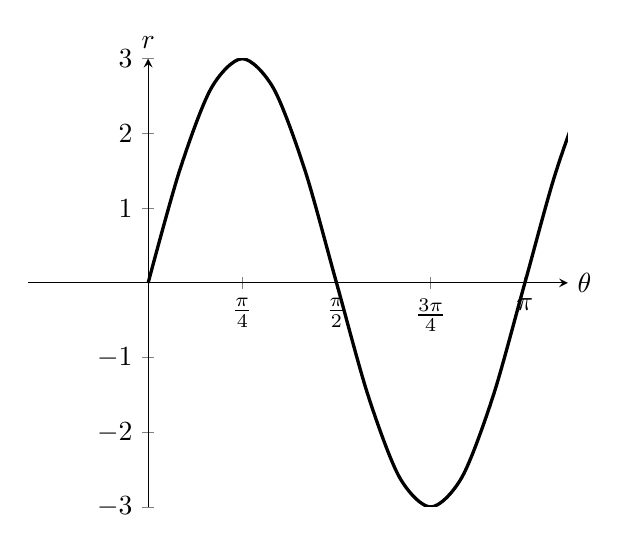
\begin{tikzpicture}  
    \begin{axis}[  
        xmin=-1,  
        xmax=3.5,  
        ymin=-3,  
        ymax=3,  
        axis lines=center,  
        xlabel=$\theta$,  
        ylabel=$r$,  
        every axis y label/.style={at=(current axis.above origin),anchor=south},  
        every axis x label/.style={at=(current axis.right of origin),anchor=west},  
       xtick={ .785, 1.57, 2.356, 3.14},
       xticklabels={ $\frac{\pi}{4}$, $\frac{\pi}{2}$, $\frac{3\pi}{4}$, $\pi$ },
       ytick={-3, -2, -1, 1, 2, 3}
      ]  
      \addplot [ very thick, mark=none,domain=0:2*pi,smooth] {3*sin(deg(2*x))};
            \end{axis}  
  \end{tikzpicture}  
\end{image} 

This picture shows us clearly how $r$, the distance from the origin varies as $\theta$ varies from $0$ to $\pi$. As $\theta$ goes from $0$ to $\frac{\pi}{4}$ we see that $r$ increases from $0$ to $3$. Then as $\theta$ varies from $\frac{\pi}{4}$ to $\frac{\pi}{2}$, we see that $r$ decreases from $3$ to $0$. This corresponds to the first lobe of the flower that lies in the 1st quadrant of the graph that uses the $x$ and $y$ axes. 


In order to evaluate the integral, recall the trig identity $sin^2(\theta)=\frac{1-\cos(2\theta)}{2}$. 


To find the entire area enclosed by the curve $r=3\sin(2\theta)$  (of all four petals) we can either use symmetry and multiply the area of one lobe by $\answer{4}$ or
we could note that the curve is traced out once by varying $\theta$ from $0$ to $2\pi$. 
This means we could integrate from $0$ to $2\pi$ to capture all the area. 







\end{hint}

\end{exercise}
\end{document}
